% Pagina di dettaglio locale

È possibile visualizzare le informazioni di un locale cliccando sul nome del locale di interesse dalla classifica.

\begin{figure}[H]
\centering
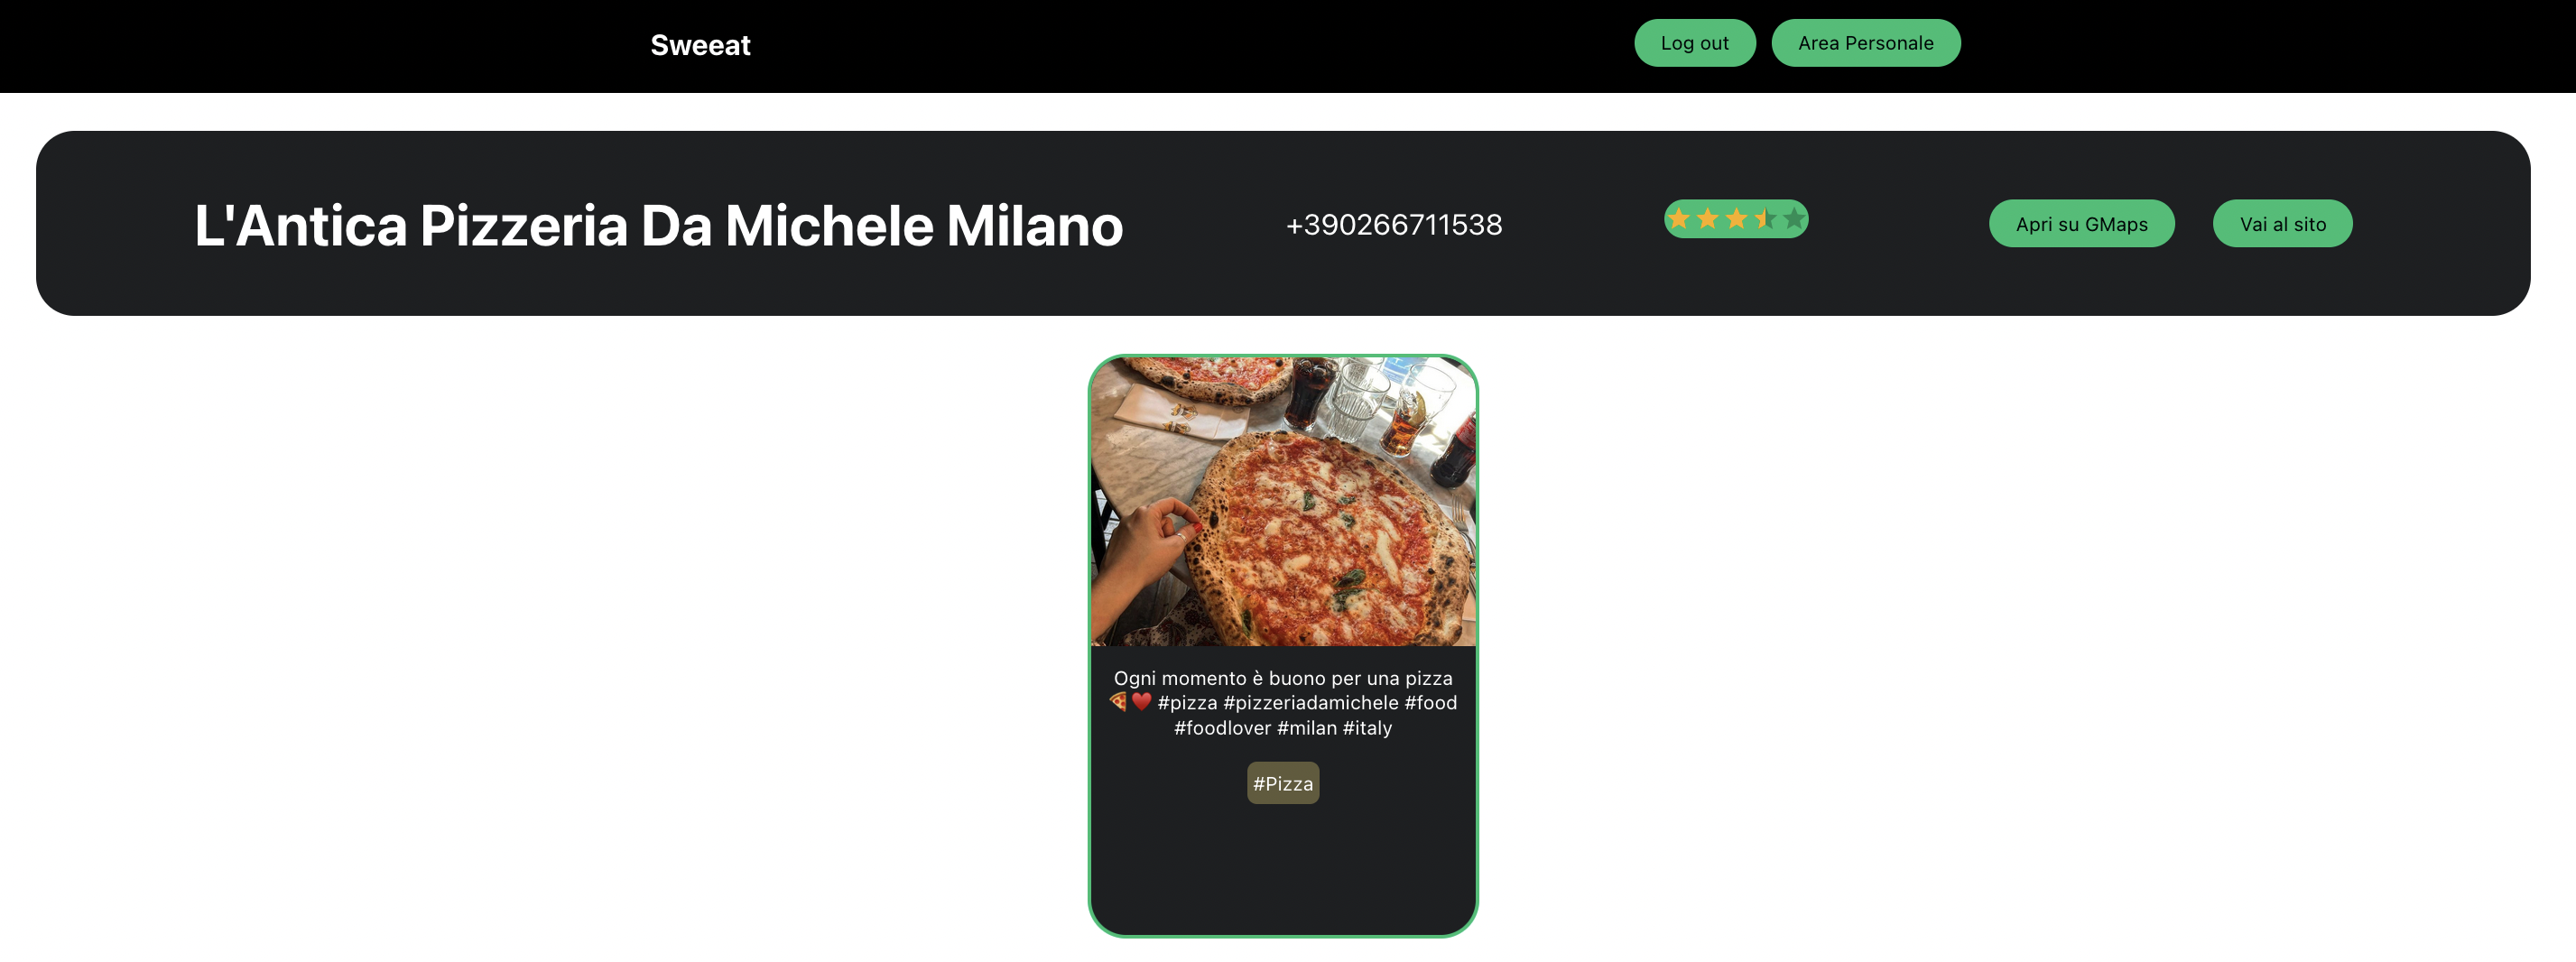
\includegraphics[scale=0.3]{./images/DettagliLocale/DettagliLocale.png} 
\caption{Pagina di dettaglio locale}
\end{figure}

Una volta cliccato sul nome del locale, all’utente verrà mostrata una nuova pagina che conterrà i seguenti dettagli:

\begin{itemize}
\item Nome locale,
\item Numero di telefono del locale,
\item Link al sito web del sito (nel caso ci sia),
\item Link alla posizizione di GMaps del locale,
\item Valutazioni:
\begin{itemize}
\item Complessiva,
\item Foto, 
\item Testo,
\item Emoji.
\end{itemize}
\end{itemize}

Inoltre, sono presenti anche uno o più post pubblicati su Instagram e relativi al locale di cui si sta visualizzando la pagina di dettaglio.
Per ciascun post vengono mostrati:

\begin{itemize}
\item Immagini del post,
\item Testo del post,
\item Tag relativi alle immagini del post.
\end{itemize}

Attualmente, viene mostrata solo la prima immagine del post.

\begin{figure}[H]
\centering
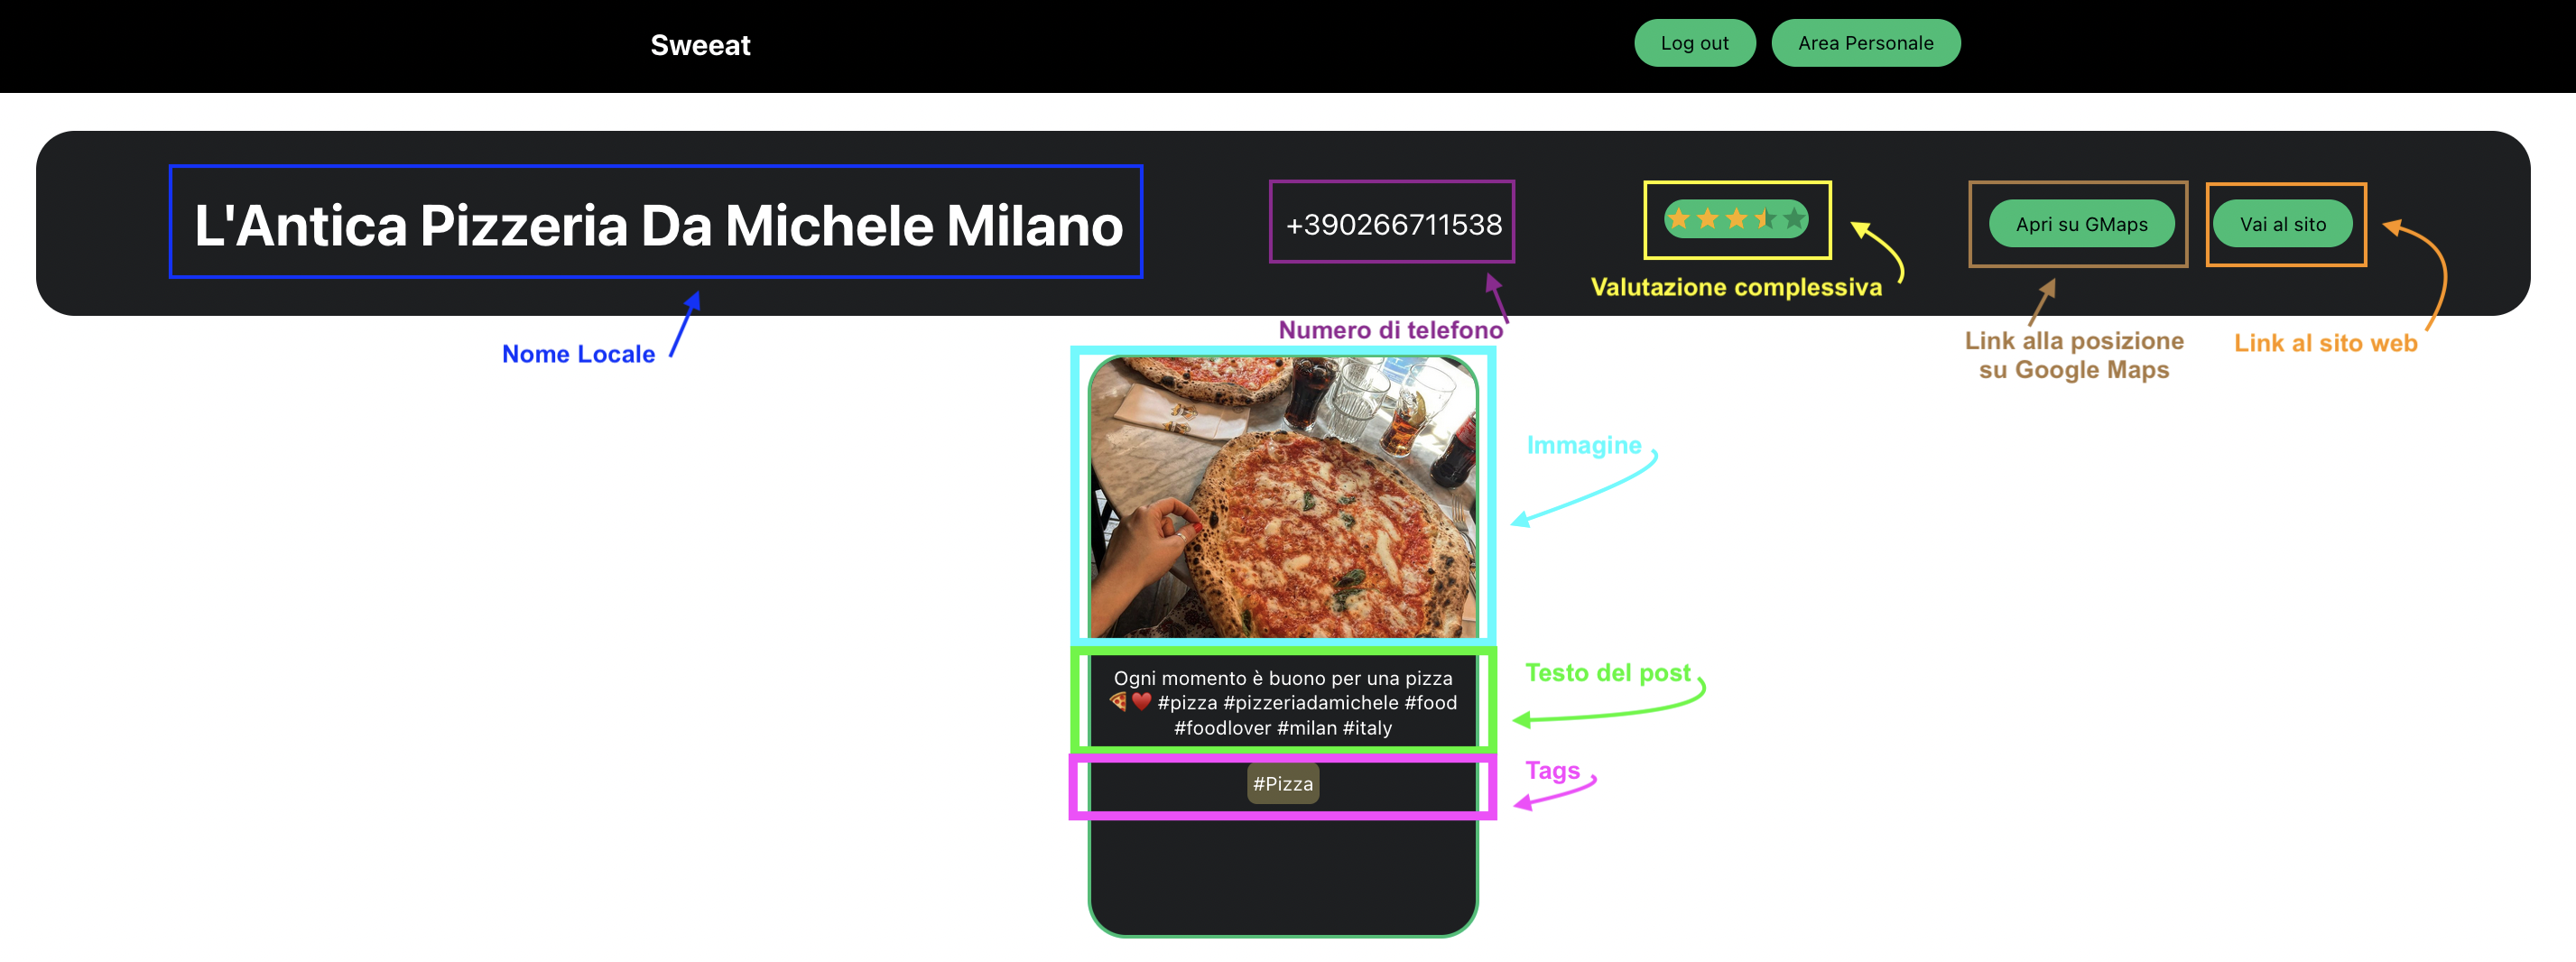
\includegraphics[scale=0.3]{./images/DettagliLocale/DettagliLocale2.png} 
\caption{Informazioni visualizzate pagina di dettaglio locale}
\end{figure}